\documentclass[a4paper,12pt]{article}
\usepackage{times}
\usepackage[francais]{babel}
\usepackage[utf8x]{inputenc}
\usepackage[T1]{fontenc}
\usepackage{amsmath}
\usepackage{amssymb}
\usepackage{graphicx}
\usepackage{pdfpages}
\usepackage{pdflscape}
\usepackage{listings}
\usepackage{longtable}
\lstset{literate=
{é}{{\'e}}1
{è}{{\`e}}1
{ê}{{\^e}}1
{à}{{\`a}}1
{â}{{\^a}}1
}
\lstset{language=C++,
                basicstyle=\footnotesize,
                keywordstyle=\footnotesize\color{blue},
                otherkeywords={override,nullptr}
}
\definecolor{orange}{rgb}{0.8,0.4,0.0}
\definecolor{darkblue}{rgb}{0.0,0.0,0.6}
\definecolor{cyan}{rgb}{0.0,0.6,0.6}
\lstdefinelanguage{JSON}
{
  basicstyle=\normalsize,
  columns=fullflexible,
  showstringspaces=false,
  commentstyle=\color{gray}\upshape,
  morestring=[b]",
  morestring=[s]{>}{<},
  morecomment=[s]{<?}{?>},
  stringstyle=\color{orange},
  identifierstyle=\color{darkblue},
  keywordstyle=\color{blue},
  morekeywords={string,number,array,object}% list your attributes here
}

\sloppy

\setlength{\topmargin}{0cm}
\setlength{\headsep}{0.in}
\setlength{\headheight}{0.in}
\setlength{\evensidemargin}{0cm}
\setlength{\oddsidemargin}{-1cm}
\textwidth 18cm
\textheight 25cm

\begin{document}

\thispagestyle{empty}

\begin{titlepage}

\vspace*{2cm}

\begin{center}\textbf{\Huge Projet Logiciel Transversal}\end{center}{\Large \par}

\begin{center}\textbf{\large WANG Zhao BENMIRA Eltadj PRADINES Louis}\end{center}{\large \par}

\vspace{2cm}

\begin{figure}[h]
\begin{center}
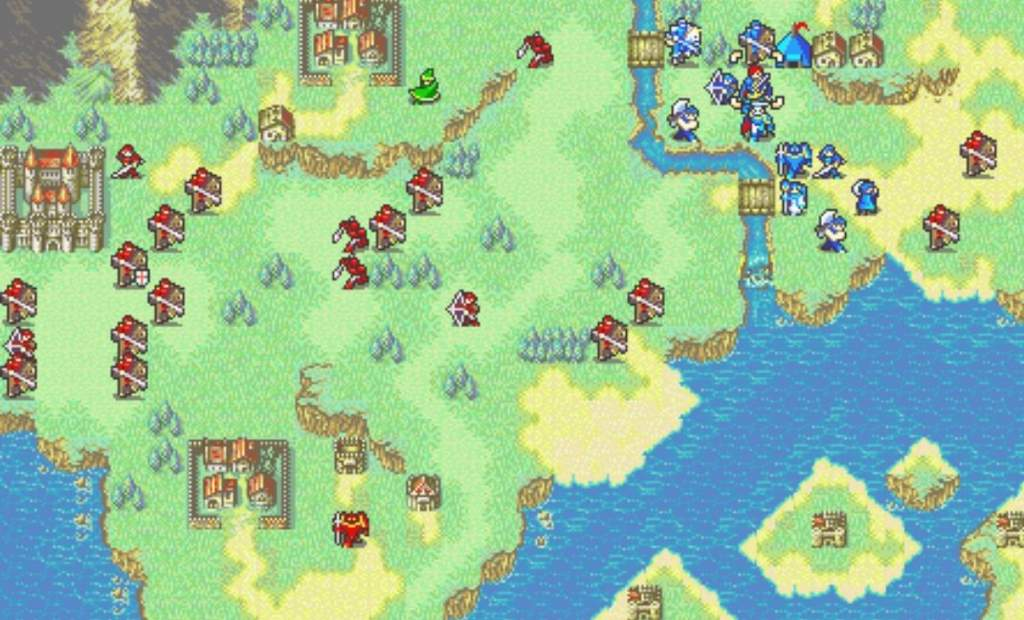
\includegraphics[width=\textwidth]{exemple.jpg}
\caption{\label{pacmangame}Exemple du jeu}
\end{center}
\end{figure}

\clearpage

{\small
\tableofcontents
}

\end{titlepage}

\clearpage
\section{Présentation Générale}

\subsection{Archétype}

L'objectif de ce projet est de réaliser un tactical RPG à la Fire Emblem, un exemple est proposé à la figure 1. Un tactical RPG est un jeu de rôle tactique. Dans ce genre de jeu vidéo, le gameplay est basé sur les décisions tactiques que le joueur doit prendre au cours des combats. Le joueur doit utiliser ses personnages pour éliminer tous les personnages ennemis du plateau, chaque personnage possède comme dans un RPG traditionnel un niveau et des statistiques qui définissent sa puissance.

\subsection{Règles du jeu}
\subsubsection{Présentation des règles}
Pour gagner la partie il faut tuer tous les personnages de l'ennemi (chaque joueur a 5 personnages). On joue au tour par tour, un tour est fini lorsque tous les personnages d’un joueur ont joué.
Un personnage doit faire ces actions dans son tour :
\begin{enumerate}
  \item se déplacer de [0 cases, maximum de distance parcourable]
  \item attaquer si il y a un ennemi dans sa portée d’attaque xor utiliser une potion xor attendre
\end{enumerate}
Chaque personnage possède des points de mouvement qu’il régénère au début de chaque tour, se déplacer sur une case consomme normalement 1 point de mouvement (ça dépend du type de case traversée). Lorsqu’il n’a plus de points de mouvements, un personnage ne peut plus se déplacer.
\subsubsection{Plateau}
Le plateau fait 17x17 cases, chaque cases possède des particularités
\begin{figure}[ht]
\begin{center}
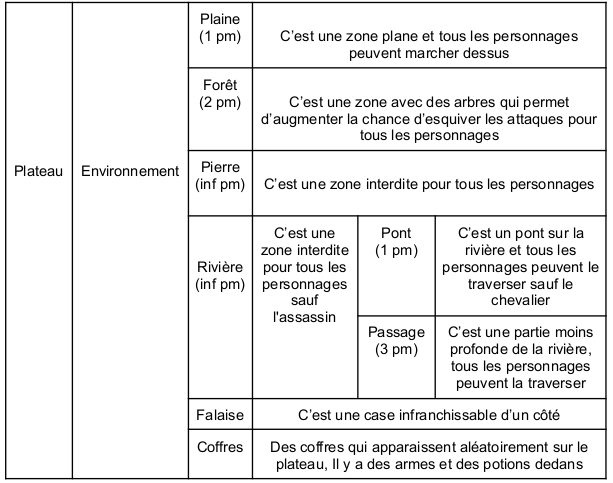
\includegraphics[width=0.7\textwidth]{tableauplateau.png}
\end{center}
\end{figure}
\newpage
\subsubsection{Saisons}
Il y a quatre saisons à la fin de chaque tour (lorsque les 2 joueurs ont joué) la saison change. Chaque saison donne des bonus généraux à tous les personnages, des bonus spécifiques aux personnages qui sont reliés à celle-ci et des malus aux personnages qui sont reliés à la saison opposée. L’ordre des saisons est le suivant: Printemps → Été → Automne → Hiver
\begin{figure}[ht]
\begin{center}
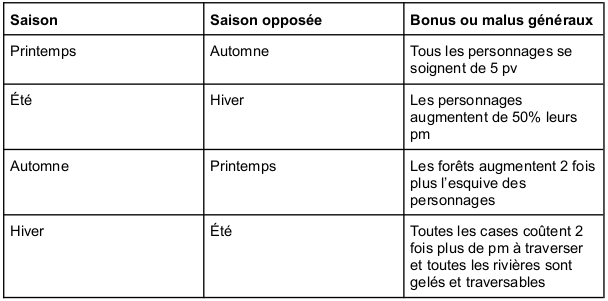
\includegraphics[width=0.7\textwidth]{tableausaison.png}
\end{center}
\end{figure}
\subsubsection{Personnages}
Chaque joueur dispose de 5 personnages (Assassin, mage, chevalier, archer et combattant). Ces personnages possèdent des armes et des spécificités liées à la saison auxquelles ils sont reliés:
\begin{figure}[ht]
\begin{center}
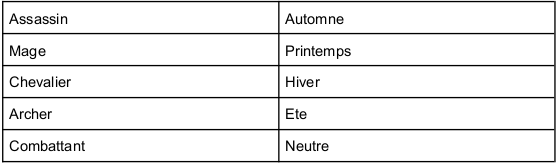
\includegraphics[width=0.7\textwidth]{tableaupersonnages.png}
\end{center}
\end{figure}
\paragraph{}
Lorsque la saison d’un personnage est effective, il reçoit des bonus  qui améliorent ses attaques et sa défense ainsi que ses déplacements.
Chaque personnage possède ses propres armes et bonus lié à sa particularité:
\paragraph{}
L' assassin: L'assassin possède une dague, il traverse les cases rivières, et un bonus est appliqué à son attaque lorsqu'il attaque par derrière. En automne sa technique est multipliée par 2. Au printemps sa technique est divisée par deux.
\paragraph{}
Le Mage: Le mage utilise la magie, il peut apporter des soins.
Au printemps le mage a la capacité de ressusciter le dernier personnage tué de son équipe. En hiver le mage perd ses pouvoirs de soin, il peut donc plus soigner aucun personnage.
\paragraph{}
Le chevalier: Le chevalier possède pour arme une épée, c'est un cavalier il a donc un grand nombre de points de déplacement. Il a pour particularité de pouvoir se déplacer après avoir attaqué (s' il lui reste des points de mouvements) mais il a pour malus de ne pas pouvoir traverser les ponts. En hiver le chevalier à la capacité d’augmenter sa défense. En été, la défense du chevalier est divisée par deux .
\paragraph{}
Archer: l’archer possède pour arme un arc et des flèches, il a pour spécificité de pouvoir augmenter sa portée d'attaque lorsqu'il est sur une case montagne.
En été sa portée augmente mais en hiver elle baisse.  
\paragraph{}
Combattant: Le combattant  a pour arme une lance par défaut au début du jeu mais il a la capacité contrairement aux autres personnages de pouvoir porter toutes les armes possible.  Il est considéré comme un personnage ‘neutre ‘ il n’a donc pas de spécificité lié aux saisons.
Le combattant possède un bonus qui lui permet d’obtenir deux fois plus d’armes à l’ouverture d’un coffre.

\subsubsection{Statistiques}
Chaque personnage possède des statistiques qui augmentent aléatoirement dès qu’il gagne un niveau
\begin{figure}[ht]
\begin{center}
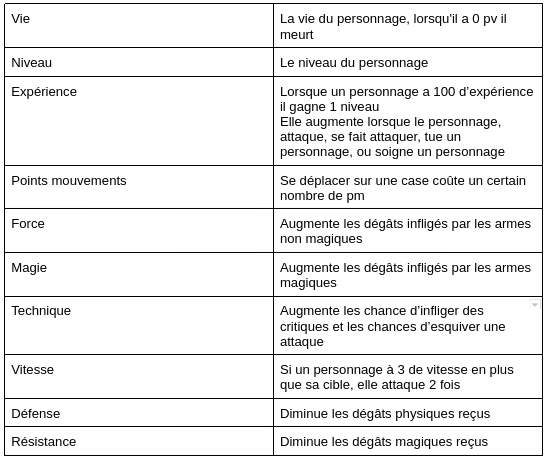
\includegraphics[width=0.7\textwidth]{tableaustats.png}
\end{center}
\end{figure}
\newpage
\subsubsection{Objets}
\begin{figure}[ht]
\begin{center}
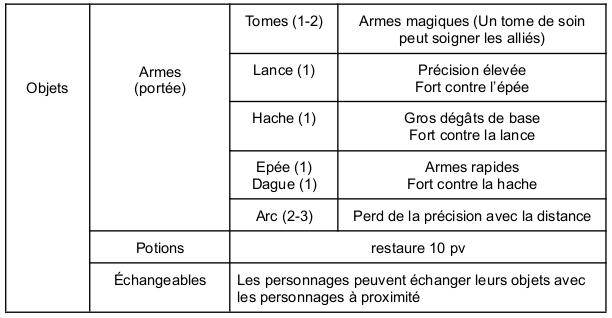
\includegraphics[width=0.7\textwidth]{tableauobjets.png}
\end{center}
\end{figure}
\subsection{Ressources}
On a besoin de textures pour les cases, une case est un carré de 128 pixels. Les textures des cases de type herbe changent de couleur en fonction des saisons
Chaque personnage a un modèle carré de 128 pixels qui le représente sur le plateau et un portrait plus détaillé qui le représente dans l'écran de statistiques, dans les dialogues,...
\begin{figure}[ht]
\begin{center}
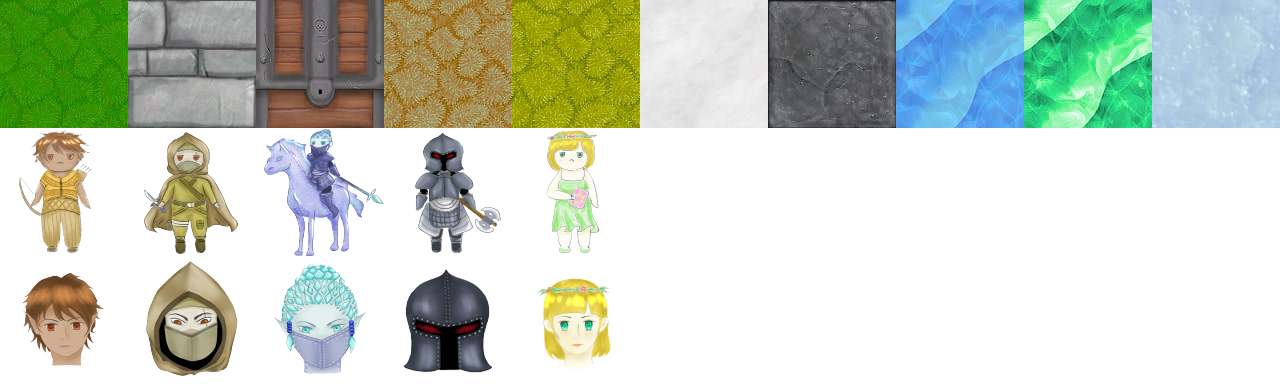
\includegraphics[width=0.7\textwidth]{textures.png}
\caption{Les textures du jeu}
\end{center}
\end{figure}
\newpage
La police du jeu est la suivante
\begin{figure}[ht]
\begin{center}
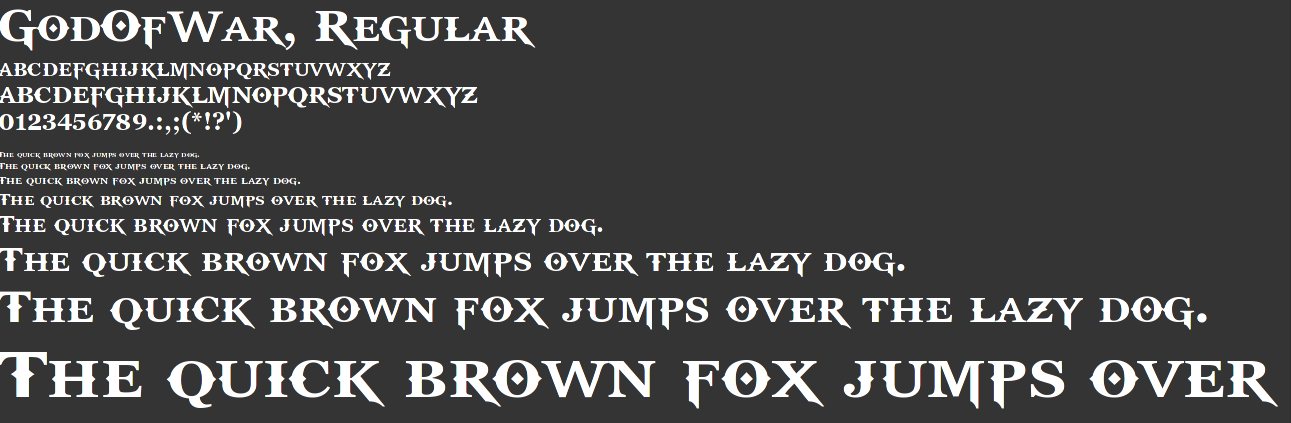
\includegraphics[width=0.7\textwidth]{ressource_police.png}
\caption{La police du jeu}
\end{center}
\end{figure}
\newpage
\subsection{Simplifications}
\paragraph{}Nous sommes un groupe de 3 et rapidement nous avons accumulé du retard sur la conception du jeu. Ainsi pour rattraper notre retard nous avons simplifié les règles du jeu.
Tout d'abord les cases n'ont plus de particularités, ie l'assassin ne peut plus traverser les cases rivières.
De plus nous avons choisi de supprimer les cases Forêt, Pierre, Falaise et Coffre.
Nous avons aussi choisi de ne pas implémenter les objets (armes et potions) et les capacités, ainsi chaque personnage a une portée d'attaque de 1. 
Pour finir nous avons aussi simplifié les saisons, les saisons accordent juste un bonus (resp. un malus) de 1 en force, technique, magie, vitesse, défense et résistance au personnage qui est de la même saison (resp. au personnage qui est de la saison opposée) et en hiver le coût en pm des cases est doublé mais on peut traverser la rivière gelé.

Les joueurs peuvent avec chaque personnage réaliser les combinaisons d'actions suivantes : 
\begin{itemize}
\item déplacer puis attaquer 
\item déplacer puis attendre
\item attaquer
\item attendre
\end{itemize}

Si un personnage attaque un autre personnage ou attend c'est au tour du personnage suivant. 
Lorsque le joueur a joué avec tous ses personnages (qui sont automatiquement sélectionnés dans l'ordre par le state) c'est au tour de l'autre joueur dès que plus aucun personnage ne peut jouer, on passe au tour suivant. 

\paragraph{} 
Désormais le jeu se joue au clavier, les touches sont les suivantes :
\begin{itemize}
\item A : attendre
\item Z,Q,S,D : se déplacer
\item UP, DOWN, LEFT, RIGHT : attaquer
\end{itemize}
\begin{figure}[ht]
\begin{center}
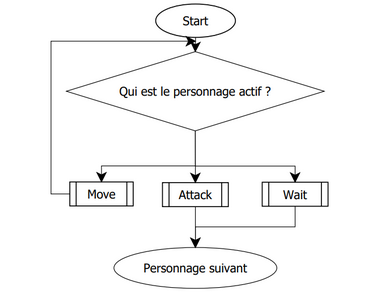
\includegraphics[width=0.6\textwidth]{phase.png}
\caption{Le déroulement d’une phase de jeu}
\end{center}
\end{figure}
\clearpage
\section{Description et conception des états}
\paragraph{} Un état du jeu est formé par un ensemble d’éléments. Tous les éléments possèdent un identifiant, un Id qui permet de connaître leur type. Cet Id permettra notamment d'afficher chaque élément.
\paragraph{} Remarque : L'id de chaque élément possède 2 chiffres, le chiffre de la dizaine indique la catégorie de l'élément, ainsi si c'est un joueur il commence par un 4, par 3 si c'est une saison, par 2 si c'est un objet, par 1 si c'est une case du plateau (cell) et par 0 si c'est un personnage. Le deuxième chiffre indique plus en détail dans quel état est l'élément.     
\subsection{Description des états}
\subsubsection{États des personnages}
Chaque personnage possède une classe, il peut être :
\begin{itemize}
\item un archer
\item un assassin
\item un mage
\item un chevalier
\item un combattant
\end{itemize}
\begin{figure}[ht]
\begin{center}
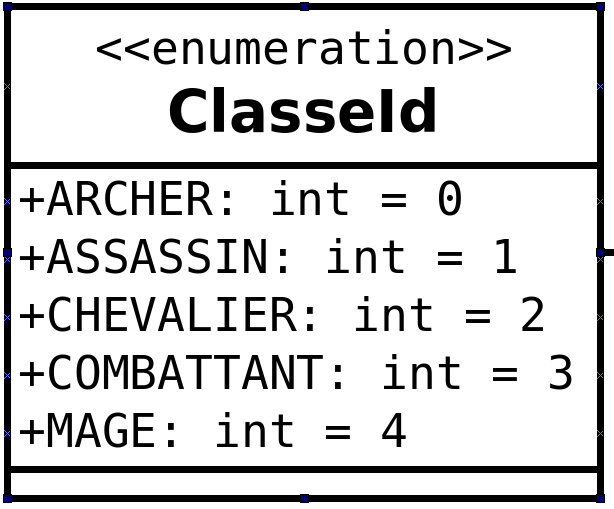
\includegraphics[width=0.2\textwidth]{classes.png}
\caption{\label{pacmangame}les Id des classes}
\end{center}
\end{figure}
\paragraph{} On associe à chacune de ces classes un Id qui lui est propre (attention plusieurs personnages peuvent avoir une même classe)
\paragraph{}Un personnage possède aussi des statistiques qui lui sont propres et qui sont stockés dans une classe Statistiques. A chaque personnage on associe 2 instances de Statistiques: une pour les statistiques brutes (statistiques avant bonus ou malus) et une pour les statistiques actuelles (après application des bonus et des malus). On remarque aussi que la classe statistique contient des attributs statistiques maximum. Ils représentent la valeur que ne peut pas dépasser les statistiques "consommables" (ie la vie, les points de mouvements et l'expérience) lorsque le personnage accomplit une action qui les influence comme par exemple se soigner en utilisant une potion.
\paragraph{} Uniquement 3 statistiques affectent l'état du personnage. Tout d'abord, la vie, en effet lorsque la vie du personnage atteint 0, celui-ci meurt et son état alive passe alors à false. Ensuite il y a les points de mouvements lorsqu' ils atteignent 0 le personnage ne peut plus se déplacer et enfin l'expérience, lorsque celle-ci atteint sa valeur maximale (définie par l'attribut experience\_max) le personnage gagne un niveau. Les autres statistiques affectent les performances du personnage en combat.
\paragraph{}En tout un personnage possède 8 statistiques influencés par les niveaux lorsqu' un personnage gagne un niveau, il a une probabilité x d'augmenter dans la statistique i. Ces probabilités sont définies par un vecteur de float : probaGainStats. Ce vecteur est propre à chaque classe.
\begin{figure}[ht]
\begin{center}
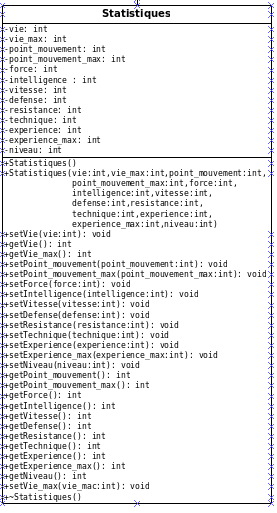
\includegraphics[width=0.5\textwidth]{statistiques.png}
\caption{\label{pacmangame}la classe Statistiques}
\end{center}
\end{figure}

\subsubsection{États des cases}
Chaque case (cell) possède un type, elle peut être :
\begin{itemize}
\item de type grass (printemps, été, automne, hiver)
\item de type river (hiver, autre)
\item de type bridge
\item de type passage
\end{itemize}
\paragraph{}Chaque type a une texture qui lui est associée lors du rendu, de plus les types modifient aussi le coût en point de mouvement que coûte la case à traverser. Ce coût varie en fonction des saisons. De plus on peut remarquer que les types grass et river changent en fonction des saisons. Pour les cases de type grass c'est un indicateur visuel pour que le joueur sache quelle est la saison du tour actuel. Pour les cases de type river, c'est pour montrer que en hiver les rivières sont gelés et donc traversables.
\begin{figure}[ht]
\begin{center}
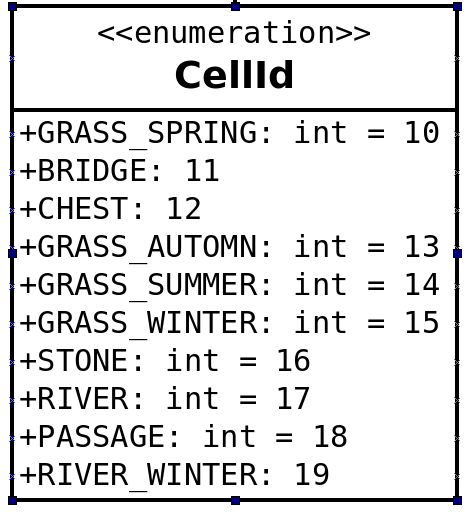
\includegraphics[width=0.2\textwidth]{cell.png}
\caption{\label{pacmangame}Les différents type de CELL(case)}
\end{center}
\end{figure}



\subsection{Conception Logiciel}
Ci dessous vous trouverez le dia du state
\newpage
\begin{landscape}
\begin{figure}[p]
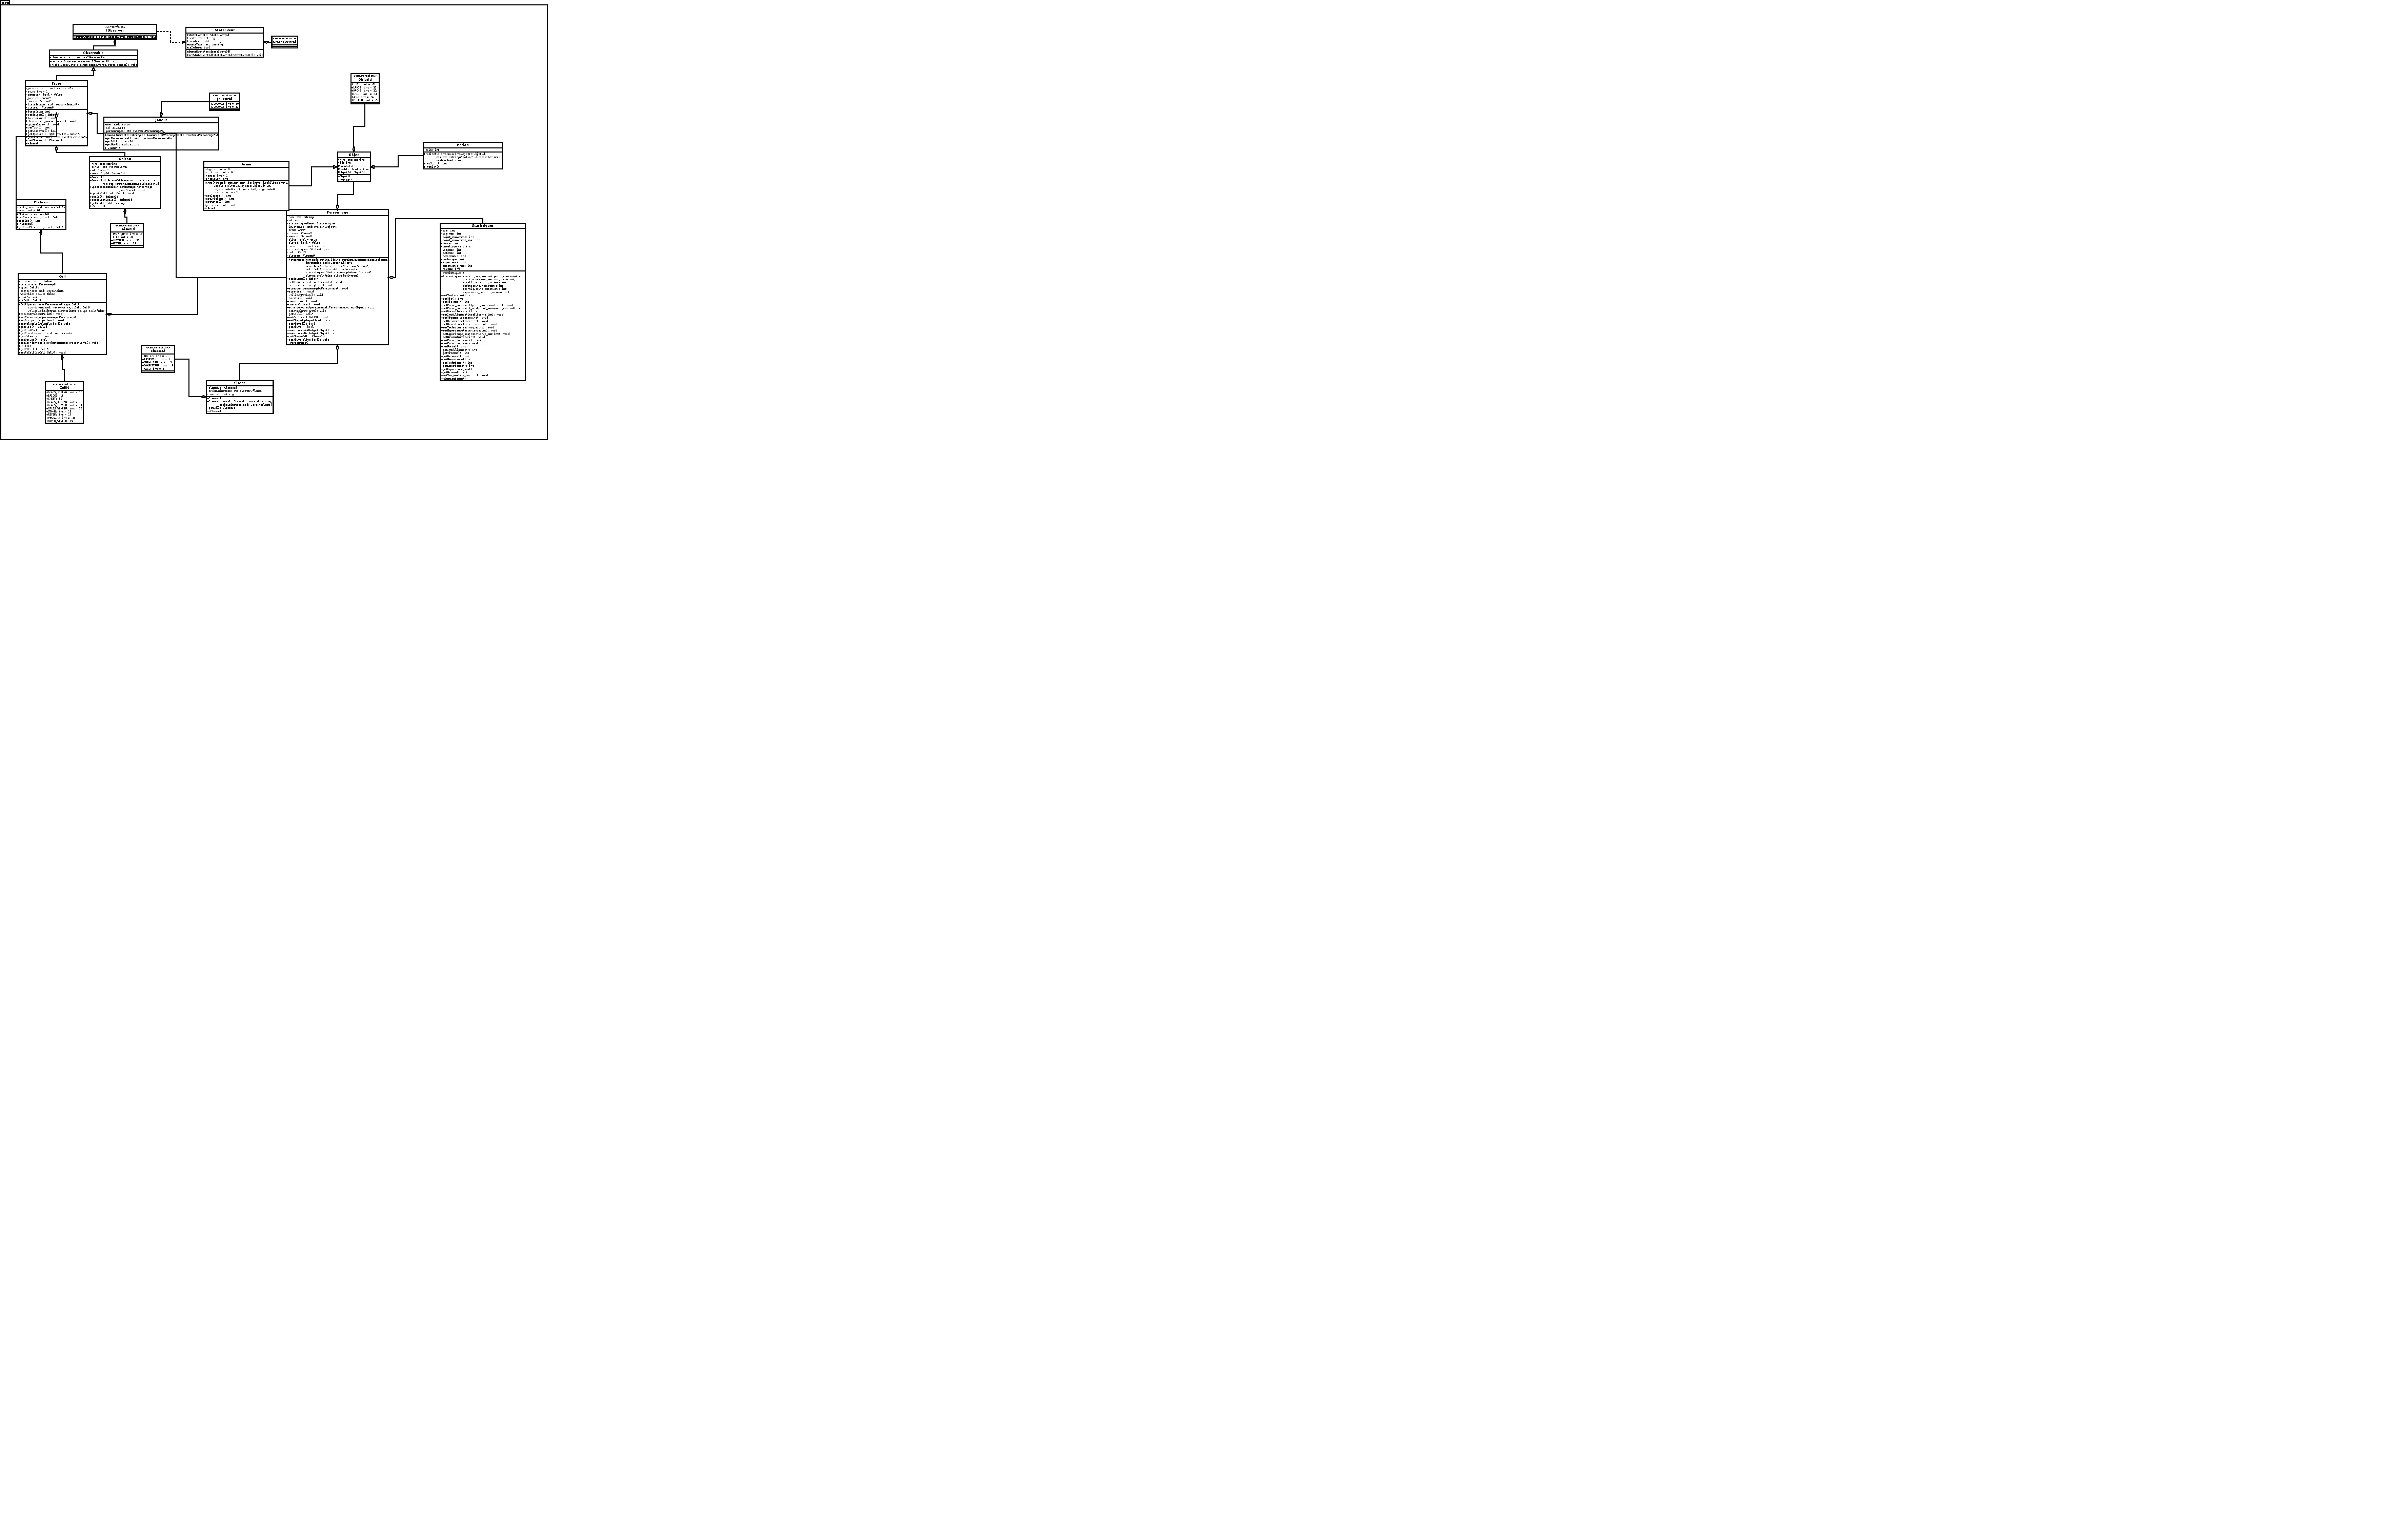
\includegraphics[width=0.6\paperheight,angle=-90]{state.pdf}
\caption{\label{uml:state}Diagramme des classes d'état.}
\end{figure}
\end{landscape}

\clearpage
\section{Rendu: Stratégie et Conception}

\subsection{Stratégie de rendu d'un état}
\paragraph{} On va utiliser une stratégie de rendu simple. On va procéder par couche. En effet, on peut facilement diviser notre jeu en 3 couches qui se superposent avec de bas en haut: le plateau, les personnages et l'interface. Plus la couche est basse, moins elle a besoin de s'actualiser fréquemment. En effet la couche Plateau doit s'actualiser une fois par tour, la couche personnage doit attendre des événements de type déplacement (le personnage bouge) ou attaque (si le personnage meurt). Tandis que la couche interface elle s'actualise pour chaque mouvement de la souris de l'utilisateur. Pour le moment notre render gère uniquement la couche plateau et la couche personnages.

\begin{figure}[ht]
\begin{center}
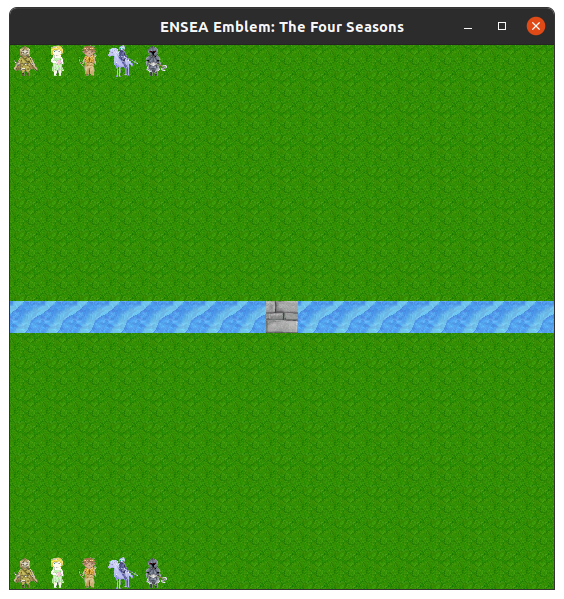
\includegraphics[width=0.7\textwidth]{render.png}
\caption{\label{pacmangame}le rendu pour 10 personnages sur un plateau de 17*17 cases}
\end{center}
\end{figure}
\newpage
\subsection{Conception logiciel}

Le rendu est composé (pour le moment car on a implémenté seulement 2 couches) de 3 classes.  

\paragraph{}La première classe StateLayer a pour objectif de récupérer du state toutes les informations utiles dont on a besoin pour afficher le rendu. Par exemple, elle doit récupérer l'Id et la position de chaque case du plateau et l'Id de la classe et la position de tous les personnages. De plus, elle doit aussi savoir quel tileset est utilisé pour chaque couche (On utilise 2 tileset, un contenant toutes les cases et un contenant tous les personnages).
\begin{figure}[ht]
\begin{center}
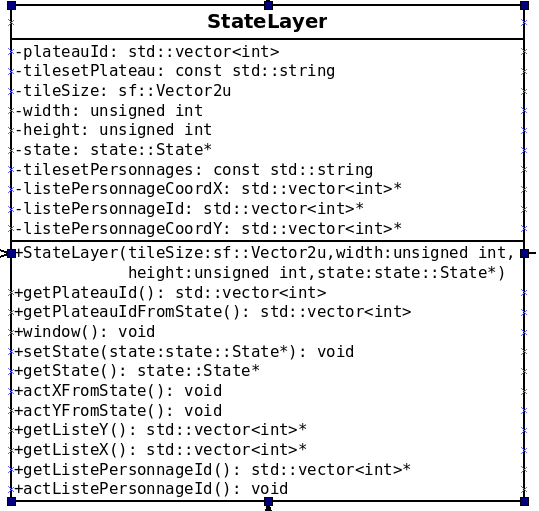
\includegraphics[width=0.6\textwidth]{statelayer.png}
\caption{\label{pacmangame}La classe StateLayer}
\end{center}
\end{figure}

\paragraph{} La classe surface elle doit utiliser toutes les informations que lui donne StateLayer pour afficher un rendu du plateau. Pour celà elle crée une liste de Vertex (dans notre cas ce sera des quads) et elle associe à chaque vertex une position dans la fenêtre du rendu et une position de texture dans le tileset. Elle à le même fonctionnement que celui décrit dans la documentation sfml (https://www.sfml-dev.org/tutorials/2.3/graphics-vertex-array-fr.php).
\begin{figure}[ht]
\begin{center}
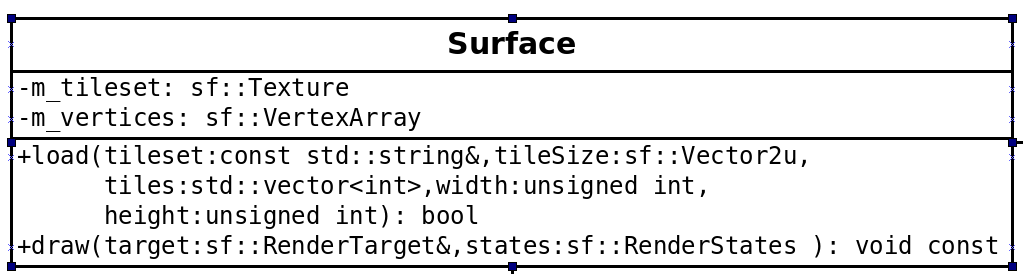
\includegraphics[width=0.6\textwidth]{surface.png}
\caption{\label{pacmangame}La classe surface}
\end{center}
\end{figure}
\newpage
\paragraph{} La classe personnage est similaire à la classe surface.

\begin{figure}[ht]
\begin{center}
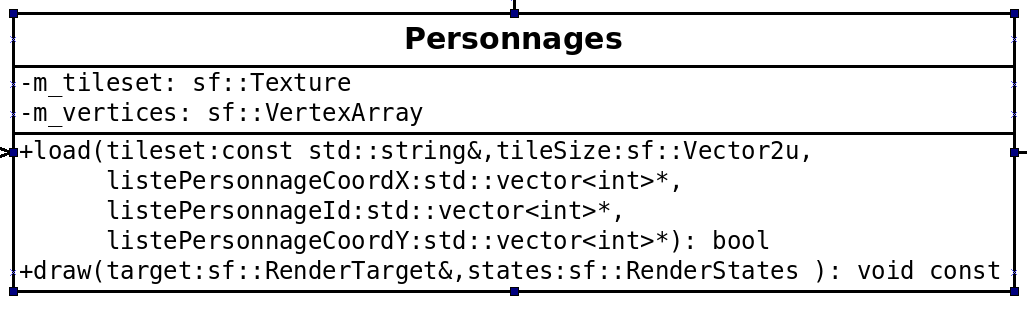
\includegraphics[width=0.6\textwidth]{personnages.png}
\caption{\label{pacmangame}La classe personnage}
\end{center}
\end{figure}


\begin{landscape}
\begin{figure}[p]
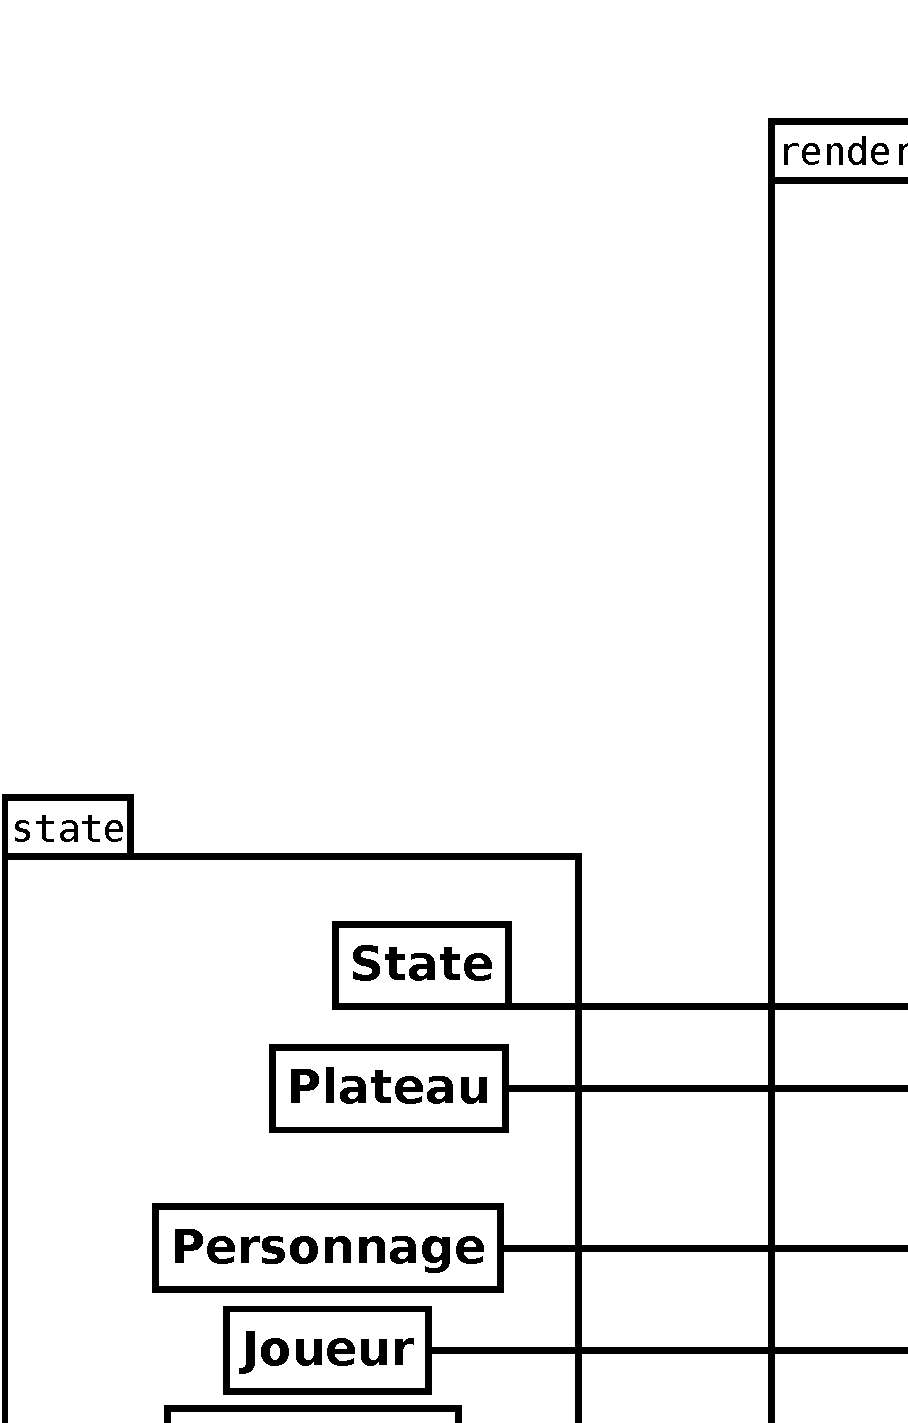
\includegraphics[width=0.7\paperheight]{render.pdf}
\caption{\label{uml:render}Diagramme des classes de rendu.}
\end{figure}
\end{landscape}

\clearpage
\section{Règles de changement d'états et moteur de jeu}
\subsection{Conception logiciel}
\paragraph{}Le diagramme des classes pour le moteur est présenté au dessous:

Le rôle des classes Commande est de lier toutes les commandes possibles dans le jeu. Pour chacune de ces classes, on défini un type de commande avec CommandId:
.\begin{itemize}
\item Commande Attaque
\item Commande Déplacer
\item Commande Échanger objet
\item Commande Attendre
\item Commande Arme
\item Commande Utilisation potion
\item Commande Fin tour
\item Commande Ouvrir coffre

\end{itemize}

La commande attaque permet lancer une attaque et de choisir une case à cibler et d'attaquer le personnage sur cette case (si il y en a un). La commande déplacer permet de déplacer un personnage dans une direction choisi, si c'est possible.La commande échanger objet permet d'échanger des objets sélectionnées lorsque deux personnages sont proches.La commande
attendre permet de faire attendre un personnage pour un tour. La commande arme permet de choisir une arme à équiper dans son inventaire. La commande utilisation potion permet au personnage de se soigner en buvant une potion, si il en a une dans son inventaire. La commande fin tour est pour faire attendre un tour tous les personnages du joueur qui active cette commande. La commande ouvrir un coffre permet à un personnage d'ouvrir un coffre si ce personnage est juste à côté de celui-ci.    

Engine est le cœur du moteur, on utilise la méthode update pour exécuter les commmandes.
\paragraph{}
Dans la classe de CommandMove, l'attribut MoveId est lié avec la classe MoveId qui gère la direction. currentState ici est pour lier avec le state.
Dans la méthode exécute de la classe CommandMove, on reçoit une direction du déplacement, et si l'endroit que le personnage active veut déplacer est bien dans le plateau, ce personnage bougera vers cette direction.

\begin{figure}[ht]
\begin{center}
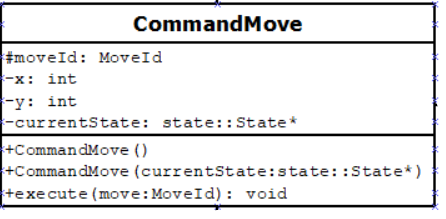
\includegraphics[width=0.6\textwidth]{CommandMove.png}
\caption{\label{pacmangame}La classe CommandMove}
\end{center}
\end{figure}

\paragraph{}
Dans la classe de CommandAtack, la méthode exécute permet de lancer la méthode attaquer dans le state, dans la classe l'engine, avant on exécute la commande attaque et lorsqu'on reçoit une direction d'attaquer, il faut d'abord vérifier l'endroit choisie est bien dans le plateau et ensuite, on détecte s'il y a un ennemie à côté du personnage active et après on exécute la commande attaque.   

\paragraph{}
Dans la classe de CommandAttendre, la méthode exécute permet de lancer la méthode attendre dans le state.
\paragraph{}
Voici un résumé du fonctionnement de l'engine :
\begin{figure}[ht]
\begin{center}
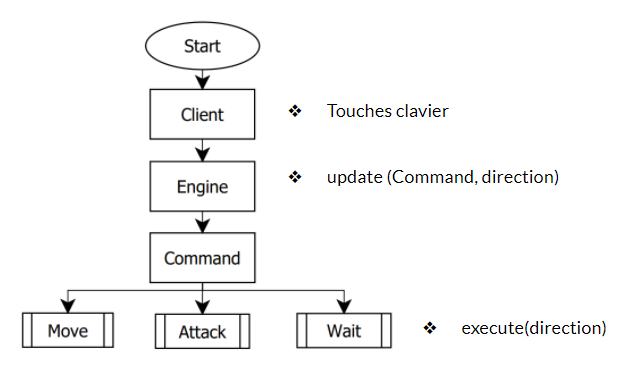
\includegraphics[width=0.6\textwidth]{resume.png}
\caption{\label{pacmangame}Résumé du fonctionnement de l'engine}
\end{center}
\end{figure}
\paragraph{}
Lorsque on lance le jeu, le client initialise le jeu. Ensuite dès qu'il reçoit une touche clavier, il l'a traduit en commande et l'envoie à l'engine qui vérifie si la commande est faisable. Si oui il modifie le state.
\newpage
\begin{landscape}
\begin{figure}[p]
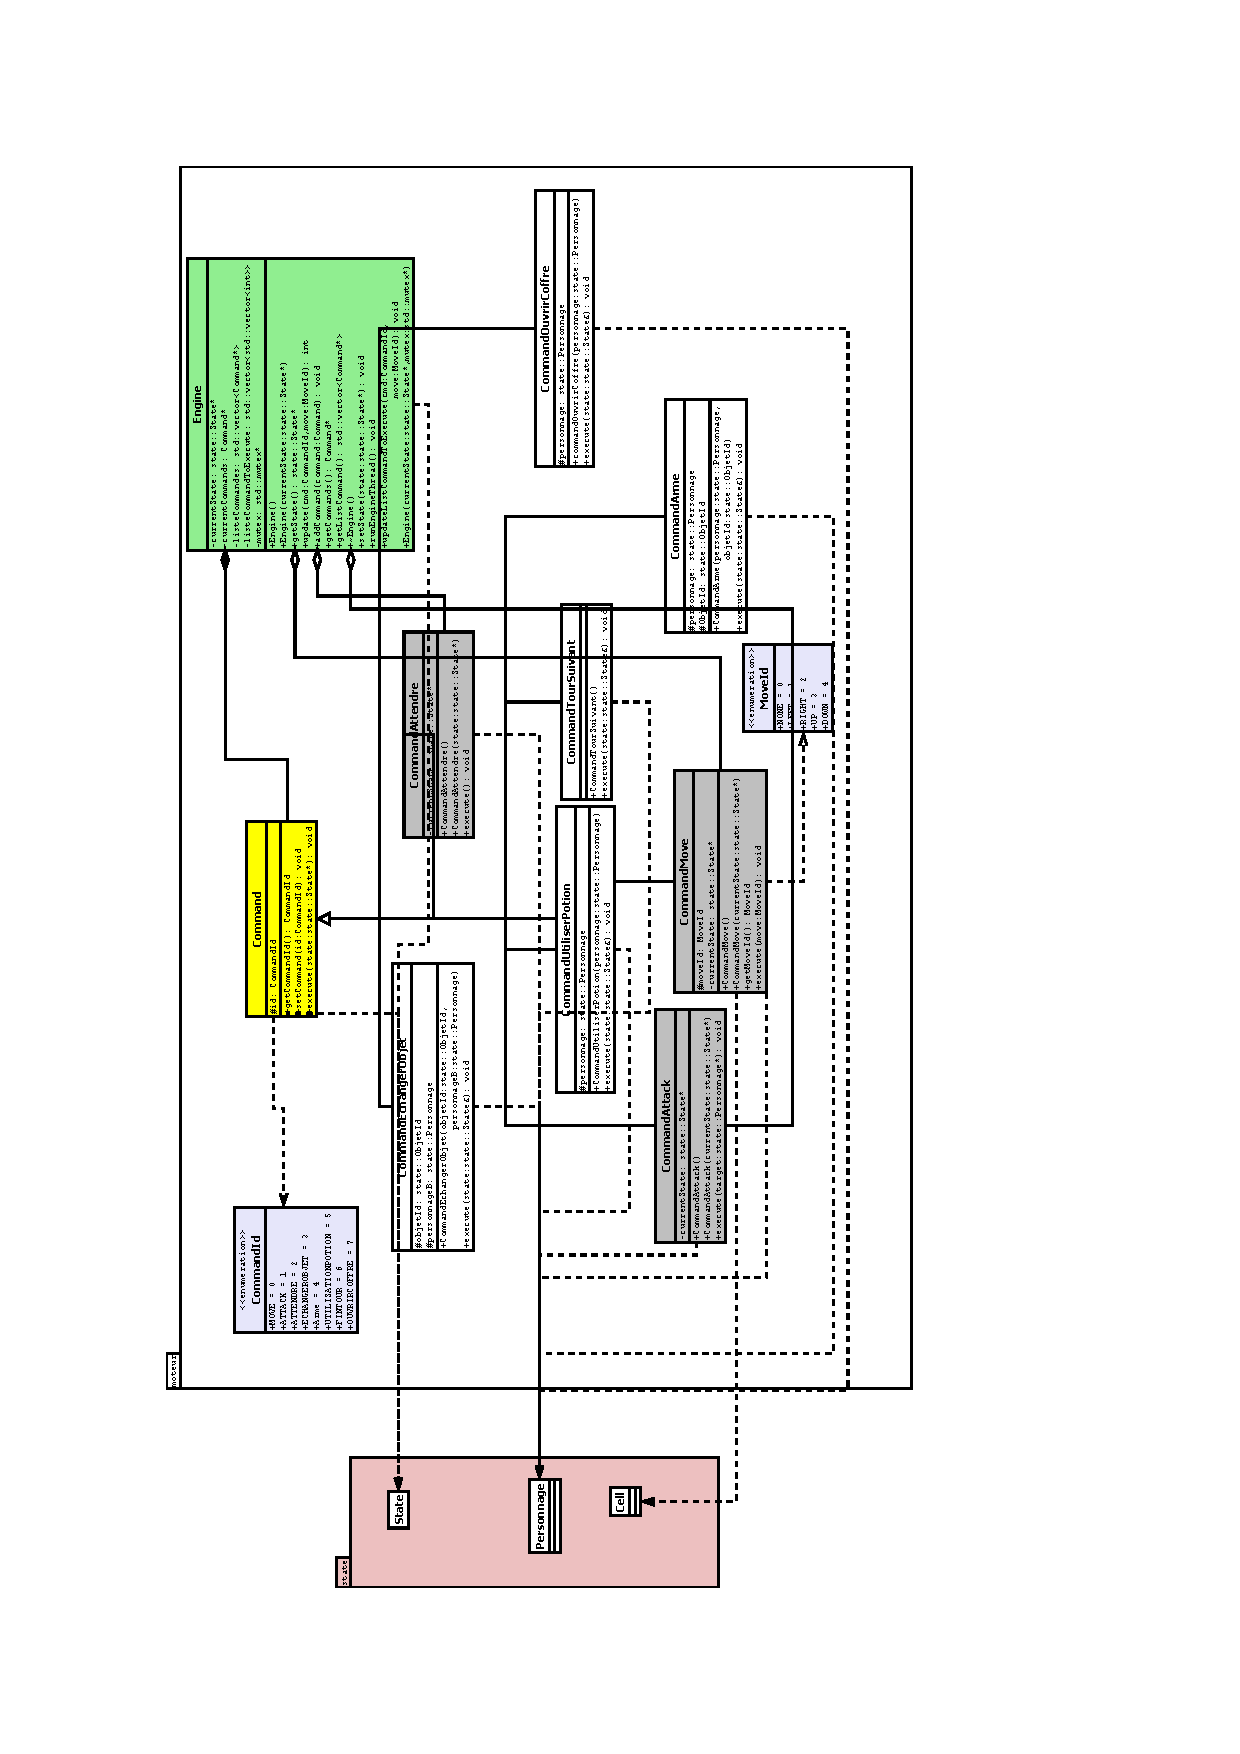
\includegraphics[width=0.6\paperheight,angle=-90]{moteur.pdf}
\caption{\label{uml:state}Diagramme des classes d'état.}
\end{figure}
\end{landscape}

\clearpage



%\begin{landscape}
%\begin{figure}[p]
%\includegraphics[width=0.9\paperheight]{engine.pdf}
%\caption{\label{uml:engine}Diagramme des classes de moteur de jeu.}
%\end{figure}
%\end{landscape}


\section{Intelligence Artificielle}

On va maintenant implémenter des intelligences artificielles, chacune aura une stratégie très différente.

\subsection{Stratégies}
\subsubsection{Intelligence aléatoire}

L'intelligence artificielle aléatoire est la plus simple de toute, sa stratégie est basée sur le diagramme suivant:
\begin{figure}[ht]
\begin{center}
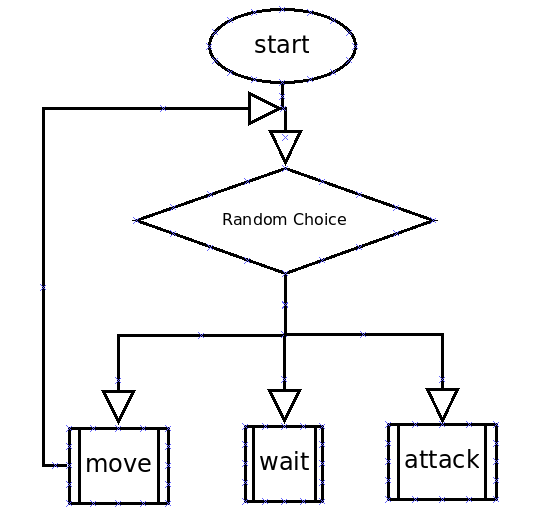
\includegraphics[width=0.6\textwidth]{iaRandomDiagram.png}
\caption{\label{pacmangame}La stratégie de l'ia aléatoire}
\end{center}
\end{figure}

Lorsque le client demande à l'ia de choisir une action à faire pour un personnage, l'ia va choisir aléatoirement si elle attaque, se déplace d'une case ou attend. Si elle choisit d'attaquer ou de bouger elle doit choisir une direction, elle va donc choisir aléatoirement 1 des 4 MoveId possible. Si la case à attaquer ou sur laquelle l'ia veut se déplacer n'est pas valide, l'engine va dire que c'est pas possible, ainsi on revient à la même situation qu'au départ et le client va à nouveau demander à l'ia de choisir aléatoirement une nouvelle commande.
Si l'ia réussit à faire bouger un personnage sur une case valide, alors elle va devoir choisir une nouvelle commande pour ce personnage. Mais si elle choisit de faire attendre le personnage ou si elle réussit à le faire attaquer un personnage alors le personnage aura finit son tour et on va passer au personnage suivant.
\begin{figure}[ht]
\begin{center}
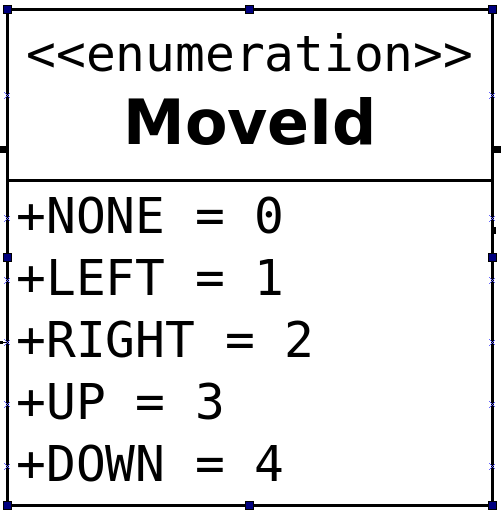
\includegraphics[width=0.3\textwidth]{moveId.png}
\caption{\label{pacmangame}La classe MoveId}
\end{center}
\end{figure}
\newpage
\subsubsection{Intelligence Heuristique}

Pour créer une intelligence artificielle un peu plus intelligente, on va rajouter des heuristiques.
Ainsi cette intelligence artificielle va regarder quel est le personnage le plus près d'elle. Ensuite elle va se déplacer vers lui, si elle est à coté de ce personnage elle va l'attaquer mais si elle n'arrive pas à se rapprocher suffisamment proche pour l'attaquer car elle a plus de point de mouvement, elle va attendre.
Si elle rencontre un obstacle sur le chemin qui est pour elle le plus court (case unwalkable ou occupée), alors elle va aussi attendre.
Pour éviter que l'IA attende devant la rivière jusqu'à ce qu'elle gèle, on rajoute une heuristique qui fait en sorte que s'il y a une rivière entre elle est le personnage le plus proche, l'ia se dirige vers le pont le plus proche.
\paragraph{} Pour tester les performances de l'IA heuristique par rapport à l'IA random. On leur fait jouer 100 parties l'une contre l'autre. L'IA heuristique gagne 91 parties, elle est donc beaucoup mieux. Les 9 parties gagnés par l'IA random sont probablement causés par l'aléatoire dans le système des dégâts (esquives). 
\subsection{Conception logiciel}

On crée une classe IA abstraite et une classe pour chaque type d'ia. Chaque type d'ia hérite de la classe IA.

\begin{landscape}
\begin{figure}[p]
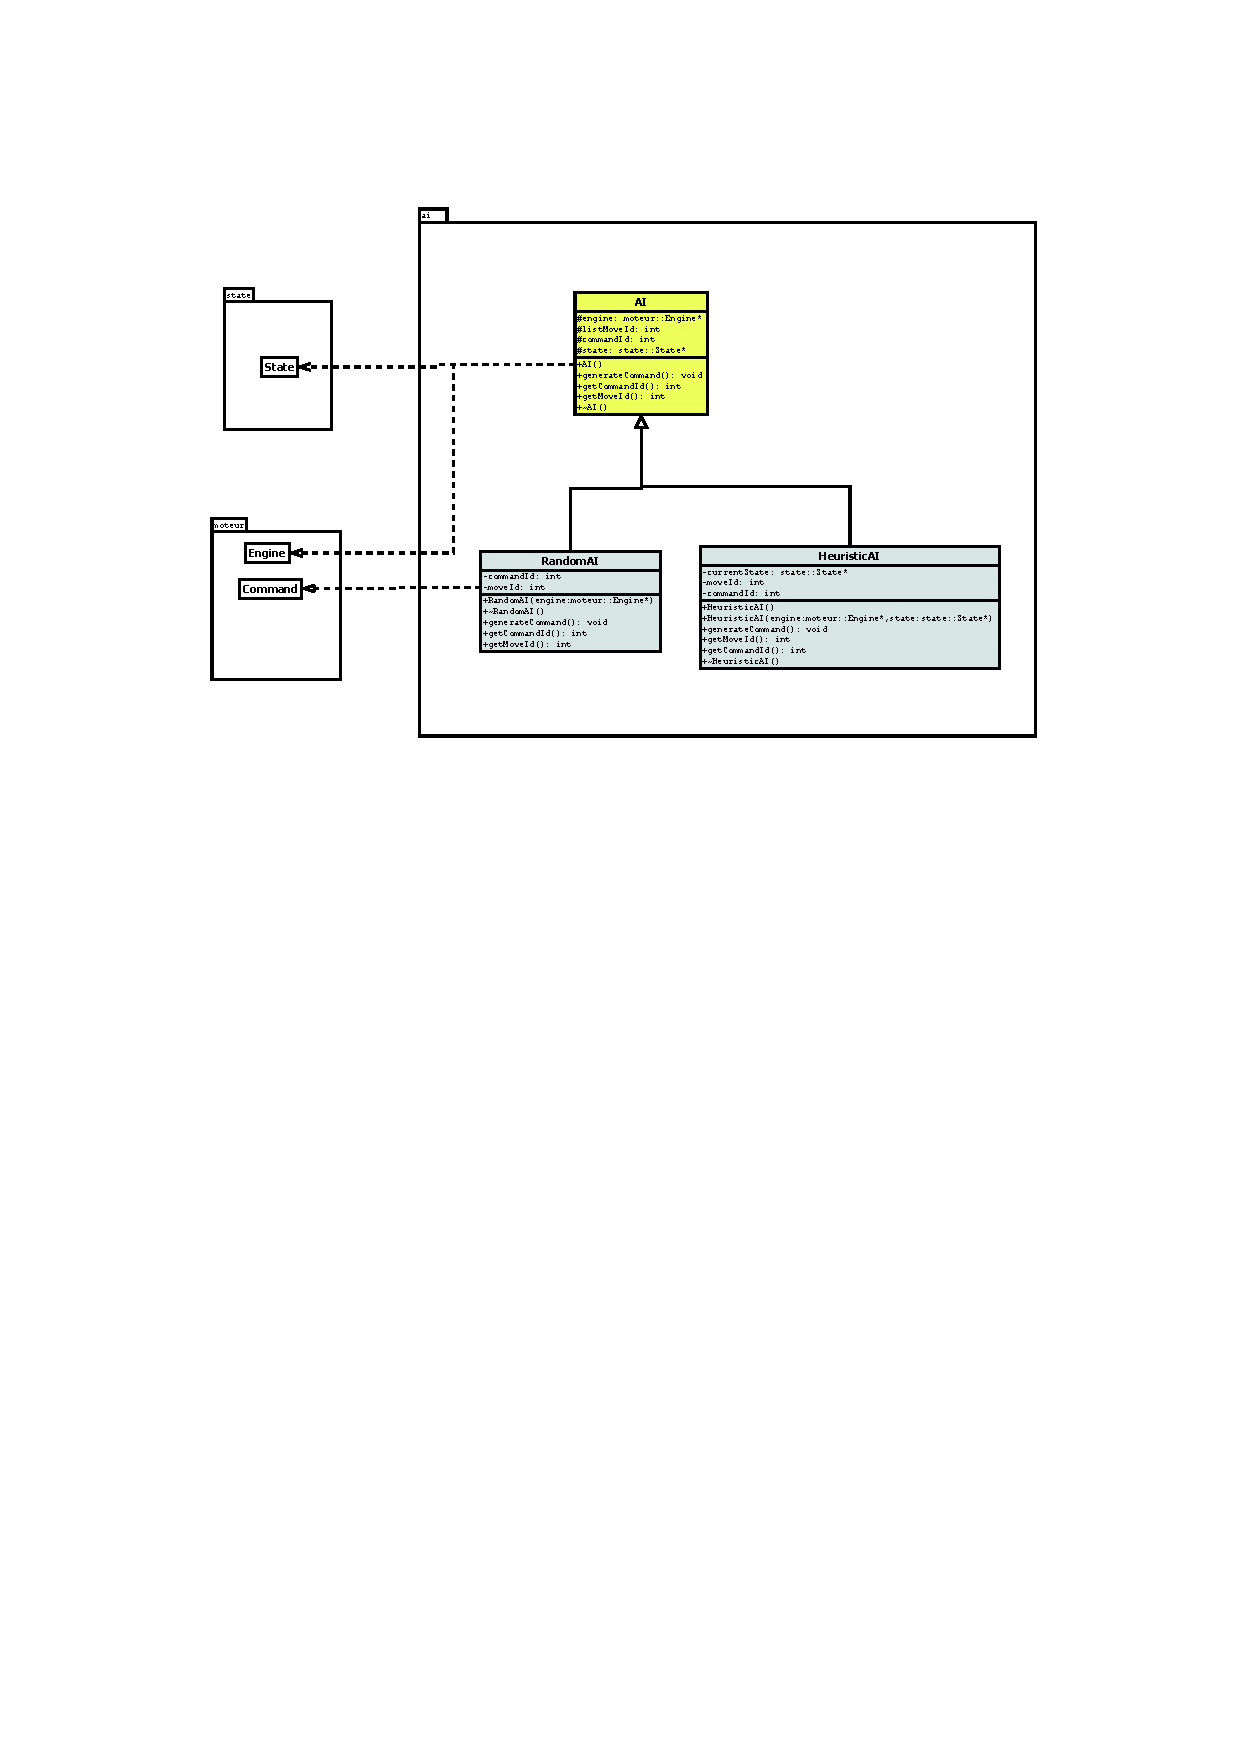
\includegraphics[width=0.9\paperheight]{ai.pdf}
\caption{\label{uml:ai}Diagramme des classes d'intelligence artificielle.}
\end{figure}
\end{landscape}

\section{Modularisation}
\label{sec:module}
\subsection{Organisation des modules}
On va diviser le jeu en 2 threads, une première thread qui va éxécuter le Client et le Render et une deuxième thread qui va éxécuter l'engine.

Pour communiquer les threads vont utiliser une liste qui va contenir la liste des commandes (une commande est définie par une liste qui contient un CommandId et un MoveId) que l'engine doit exécuter. Cette liste est protégée par un mutex. Le thread engine exécute toujours le premier élément de la liste. Dès qu'il a exécuté la commande l'engine va supprimer cette commande de la liste.
\begin{figure}[ht]
\begin{center}
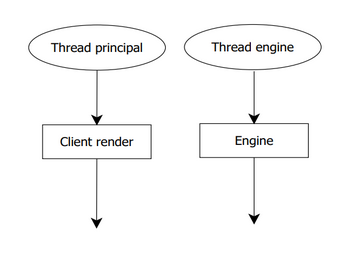
\includegraphics[width=0.7\textwidth]{thread.png}
\caption{\label{pacmangame}Le schéma des threads}
\end{center}
\end{figure}
\newpage
Ainsi la nouvelle classe engine adaptée au multithreading ressemble à ça

\begin{figure}[ht]
\begin{center}
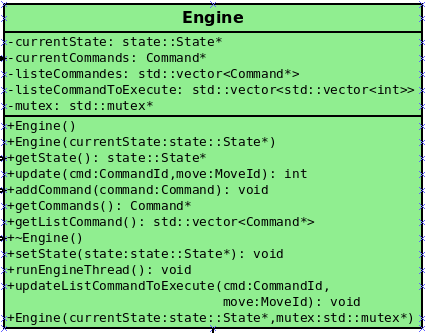
\includegraphics[width=0.7\textwidth]{enginethread.png}
\caption{La nouvelle classe engine}
\end{center}
\end{figure}

\end{document}



